\subsection{Regression-trained networks and cross-target ordering}

The regression-trained networks rank less well than the hit-head networks (Table~\ref{tab:wt}, Figure~\ref{fig:wt}). Recall in this subsection is the top-1\% recall within the best 10\% of the ranking. The geometry network recovers \wtRTestRsgWt{} with wild-type training and \wtRTestRsgInt{} with interventional training, the residue-sum network without geometry \wtRTestRsWt{}, the network with an edit record \wtRTestRseWt{} and the dual encoder trained with the present recipe \wtRTestBfiveWt{}. The geometry network exceeds the geometry-free network by \wtdTestRsgWtMinusRsWt{} (interval \wtdLoTestRsgWtMinusRsWt{} to \wtdHiTestRsgWtMinusRsWt{}) on the test targets and by \wtdDevRsgWtMinusRsWt{} (\wtdLoDevRsgWtMinusRsWt{} to \wtdHiDevRsgWtMinusRsWt{}) on the development targets. Interventional training lifts the geometry-free network (\wtRTestRsWt{} to \wtRTestRsInt{}, interval of the difference \wtdLoTestRsIntMinusRsWt{} to \wtdHiTestRsIntMinusRsWt{}) and leaves the geometry network at the level of wild-type training (\wtdTestRsgIntMinusRsgWt{}, interval \wtdLoTestRsgIntMinusRsgWt{} to \wtdHiTestRsgIntMinusRsgWt{}), so the test gain of the descriptors is not specific to them. The hit head adds \hndTestRsghWtMinusRsgWt{} and \hndTestRsghIntMinusRsgInt{} to the two geometry networks, with 34,627 additional parameters.

The reversal accuracy measures the ordering of ligand pairs whose order flips between two targets. The hit logit of the hit-head networks reproduces both orderings in \hnJDevRsghWt{} and \hnJDevRsghInt{} of the development quadruplets and \hnJTestRsghWt{} and \hnJTestRsghInt{} of the test quadruplets, and the baseline surrogates with the plain, the within-target ranking and the cross-target ranking objective reach \hitJDevCZero{}, \hitJDevCOne{} and \hitJDevCTwo{} on the development targets and \hitJTestCZero{}, \hitJTestCOne{} and \hitJTestCTwo{} on the test targets (the last objective at a recall of \hitRTestCTwo{}). A model that ranks ligands identically in every target scores zero, as the constant pocket does, and a random model scores 0.25. The score head of the hit-head networks reaches \hnScoreJDevRsghWt{} and \hnScoreJDevRsghInt{} on the development quadruplets, and the regression-trained geometry networks \wtJDevRsgWt{} (range over \wtNDevRsgWt{} seeds \wtJminDevRsgWt{} to \wtJmaxDevRsgWt{}) and \wtJDevRsgInt{} (\wtJminDevRsgInt{} to \wtJmaxDevRsgInt{}), against \wtJDevRsgShmTwo{} and \wtJDevRsgShaTwo{} for the controls with deranged labels. The test targets show a smaller effect: the geometry networks reproduce both orderings in \wtJTestRsgWt{} and \wtJTestRsgInt{} of the test quadruplets and the controls in \wtJTestRsgShmTwo{} and \wtJTestRsgShaTwo{}. A boosting model on ligand descriptors and the ten pocket descriptors reaches \wtJDevBoostGeo{} on the development quadruplets and a recall of \wtRDevBoostGeo{}, against \wtJDevBoostLig{} and \wtRDevBoostLig{} without the pocket descriptors and \wtJDevRsgInt{} for the geometry network trained on measured changes.

\begin{table}[t]
\caption{Wild-type screening and cross-target ordering. Top-1\% recall within the best 10\% of the ranking (macro average over targets; 95\% interval from bootstrapping targets) and reversal accuracy, the fraction of quadruplets of two ligands and two targets in which both opposite orderings are reproduced (mean over seeds with range). The baseline surrogates have two readouts. The hit-probability head ranked ligands in the preceding analysis (values taken from its result files), the regression head gives the predicted score that is used for the edits in this study. The development split holds 10 targets and 10{,}025 quadruplets, the test split 9 targets and 3{,}536 quadruplets. Recall of the hit-head networks is the mean of single networks, and the test labels were read once for all models except these networks and once more for them (a third read served the six networks of the comparison with joint networks, Table~\ref{tab:si_joint_runs}).}
\label{tab:wt}
\centering
\resizebox{\textwidth}{!}{%
\begin{tabular}{lrrrrrr}
\toprule
& \multicolumn{3}{c}{Development targets} & \multicolumn{3}{c}{Test targets} \\
\cmidrule(lr){2-4}\cmidrule(lr){5-7}
Model & Recall & 95\% interval & Reversal & Recall & 95\% interval & Reversal \\
\midrule
\multicolumn{7}{l}{\emph{Baseline surrogates, hit-probability head (readout of the preceding analysis)}} \\
\quad Plain objective & 0.75 & 0.55 to 0.89 & 0.01 (0.00 to 0.01) & 0.83 & 0.81 to 0.85 & 0.03 (0.02 to 0.03) \\
\quad Within-target ranking & 0.74 & 0.54 to 0.88 & 0.01 (0.01 to 0.02) & 0.78 & 0.76 to 0.81 & 0.04 (0.03 to 0.06) \\
\quad Cross-target ranking & 0.70 & 0.55 to 0.82 & 0.07 (0.02 to 0.16) & 0.63 & 0.59 to 0.67 & 0.12 (0.08 to 0.18) \\
\quad Plain objective, constant pocket & 0.74 & 0.56 to 0.88 & 0.00 (0.00 to 0.00) & 0.82 & 0.79 to 0.86 & 0.00 (0.00 to 0.00) \\
\quad Ligand-only fingerprint model (CatBoost) & 0.68 & 0.54 to 0.80 & 0.00 (0.00 to 0.00) & 0.70 & 0.67 to 0.74 & 0.00 (0.00 to 0.00) \\
\midrule
\multicolumn{7}{l}{\emph{Baseline surrogates, regression head (readout used for edits)}} \\
\quad Plain objective & 0.71 & 0.53 to 0.84 & 0.01 (0.00 to 0.01) & 0.73 & 0.71 to 0.76 & 0.06 (0.04 to 0.08) \\
\quad Within-target ranking & 0.72 & 0.55 to 0.85 & 0.02 (0.01 to 0.04) & 0.73 & 0.69 to 0.77 & 0.05 (0.04 to 0.07) \\
\quad Cross-target ranking & 0.69 & 0.54 to 0.82 & 0.02 (0.01 to 0.02) & 0.70 & 0.68 to 0.72 & 0.05 (0.04 to 0.07) \\
\quad Plain objective, constant pocket & 0.70 & 0.54 to 0.83 & 0.00 (0.00 to 0.00) & 0.74 & 0.70 to 0.79 & 0.00 (0.00 to 0.00) \\
\midrule
\multicolumn{7}{l}{\emph{Wild-type training only}} \\
\quad Dual encoder & 0.70 & 0.54 to 0.83 & 0.01 (0.01 to 0.02) & 0.72 & 0.69 to 0.75 & 0.03 (0.02 to 0.03) \\
\quad ResidueSum & 0.74 & 0.58 to 0.86 & 0.09 (0.06 to 0.13) & 0.67 & 0.61 to 0.72 & 0.07 (0.05 to 0.09) \\
\quad ResidueSum-Edit & 0.75 & 0.60 to 0.86 & 0.44 (0.34 to 0.57) & 0.81 & 0.76 to 0.86 & 0.11 (0.10 to 0.12) \\
\quad ResidueSum-Geo & 0.74 & 0.58 to 0.86 & 0.25 (0.10 to 0.37) & 0.80 & 0.76 to 0.84 & 0.12 (0.10 to 0.18) \\
\midrule
\multicolumn{7}{l}{\emph{Interventional training}} \\
\quad Dual encoder & 0.69 & 0.54 to 0.82 & 0.01 (0.00 to 0.01) & 0.73 & 0.69 to 0.77 & 0.02 (0.01 to 0.03) \\
\quad ResidueSum & 0.74 & 0.53 to 0.89 & 0.04 (0.03 to 0.04) & 0.79 & 0.75 to 0.83 & 0.04 (0.04 to 0.06) \\
\quad ResidueSum-Edit & 0.74 & 0.58 to 0.86 & 0.28 (0.26 to 0.31) & 0.80 & 0.74 to 0.84 & 0.10 (0.09 to 0.11) \\
\quad ResidueSum-Geo & 0.74 & 0.60 to 0.85 & 0.41 (0.37 to 0.49) & 0.78 & 0.73 to 0.82 & 0.10 (0.09 to 0.11) \\
\midrule
\multicolumn{7}{l}{\emph{Network with a hit head, hit-logit readout (addendum 7)}} \\
\quad ResidueSum-Geo with hit head, wild type only & 0.80 & 0.65 to 0.90 & 0.18 (0.07 to 0.32) & 0.83 & 0.80 to 0.86 & 0.04 (0.03 to 0.07) \\
\quad ResidueSum-Geo with hit head, measured changes & 0.78 & 0.62 to 0.90 & 0.08 (0.05 to 0.09) & 0.84 & 0.81 to 0.88 & 0.04 (0.03 to 0.04) \\
\midrule
\multicolumn{7}{l}{\emph{Label controls}} \\
\quad Labels permuted over ligands & 0.75 & 0.60 to 0.87 & 0.19 (0.08 to 0.28) & 0.81 & 0.77 to 0.85 & 0.08 (0.06 to 0.09) \\
\quad Labels deranged over edits (v2) & 0.75 & 0.61 to 0.85 & 0.27 (0.23 to 0.29) & 0.80 & 0.75 to 0.84 & 0.08 (0.07 to 0.09) \\
\quad All labels deranged (v2) & 0.75 & 0.60 to 0.86 & 0.15 (0.11 to 0.20) & 0.80 & 0.75 to 0.84 & 0.08 (0.07 to 0.09) \\
\bottomrule
\end{tabular}}
\end{table}


\begin{figure}[!ht]
\centering
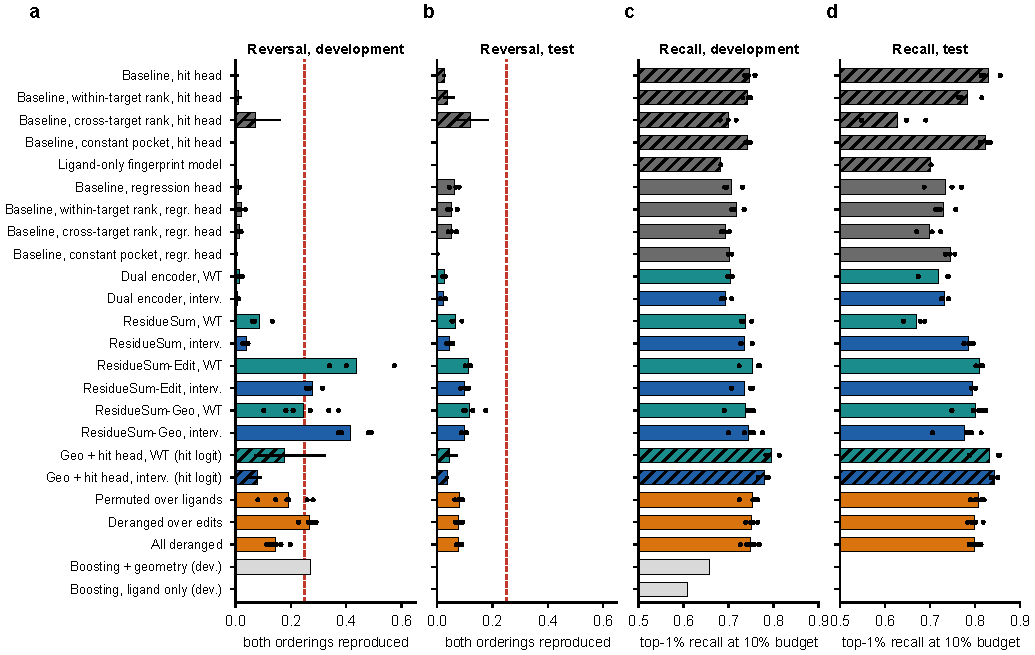
\includegraphics[width=\linewidth]{figures/fig6_wt}
\caption{Wild-type screening and cross-target ordering. Reversal accuracy (a, b) and top-1\% recall at a 10\% budget (c, d) on the development targets (a, c) and the test targets (b, d). Bars give the mean over seeds and dots single seeds. Hatched bars are the baseline surrogates read out with their hit-probability head, the readout of the preceding analysis (dots: seeds; line: range of the reversal accuracy over seeds); the regression head of the same checkpoints is shown below them. The dashed line marks random ordering in the reversal test. The descriptor models were evaluated on the development targets only. The recall axes start at 0.5.}
\label{fig:wt}
\end{figure}
